\documentclass[../../main.tex]{subfiles}
\begin{document}
\setcounter{chapter}{1}
\setcounter{section}{0}
\section{Introduction}

\textcolor{red}{**********Sit in introduction*************}

It is possible to derive a system of partial differential equations with corresponding boundary conditions but due to the complexity of the system, a different approach is considered. Consider the model problem in variational form. 

We consider the {\bf variational form} of the vibration problem. This variational problem may be used to implement the {\bf finite element method}. The finite element method can be used to simulate vibrations of the elastic body for both dynamic and static problems and also calculate the natural frequencies and modes of the elastic body. Existence and uniqueness of solutions to the problem can also be investigated using a weak version of the variational form.

\subsubsection*{A Dynamic Problem}
Find a vector valued function $u \in C(\Omega)$ such that it satisfies the equations of motion and the constitutive equations. Since $u \in C(\Omega)$, $u$ satisfies the boundary conditions defined on $\Sigma$ and $\Gamma$.\\

Initial conditions for $u$ will need to be defined.

\subsubsection*{A Static Problem}
The static porblem is a special case of the dynamic problem  where $\partial_t^2 u = 0$. In this case, there are also no initial conditions.\\
\textcolor{red}{**************************}

\textcolor{red}{Research into the behaviour of suspension bridges is still a widely researched field by both engineers and mathematicians. This research started as several bridges suffered collapse. }


\subsubsection{Different Research Approaches}
\begin{figure}[h!]
	\centering
	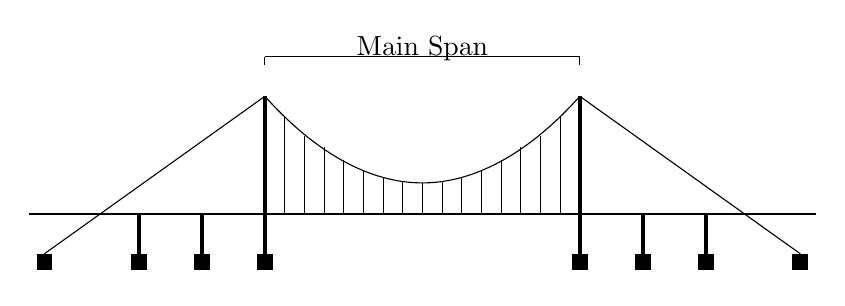
\begin{tikzpicture}
		\draw (3,2) -- (7,2);
		\draw (3,2) -- (3,1.9);
		\draw (7,2) -- (7,1.9);
		\node at (5,2.1) {Main Span};
		
		\draw[line width = 0.25mm] (0,0) -- (10,0);
		
		\draw[line width = 0.5mm] (1.4,0) -- (1.4,-0.5);
		\draw[line width = 2mm] (1.4,-0.5) -- (1.4,-0.7);
		
		\draw[line width = 0.5mm] (2.2,0) -- (2.2,-0.5);
		\draw[line width = 2mm] (2.2,-0.5) -- (2.2,-0.7);
		
		\draw[line width = 0.5mm] (8.6,0) -- (8.6,-0.5);
		\draw[line width = 2mm] (8.6,-0.5) -- (8.6,-0.7);
		
		\draw[line width = 0.5mm] (7.8,0) -- (7.8,-0.5);
		\draw[line width = 2mm] (7.8,-0.5) -- (7.8,-0.7);
		
		\draw[line width = 0.5mm] (3,1.5) -- (3,-0.5);
		\draw[line width = 2mm] (3,-0.5) -- (3,-0.7);
		
		\draw[line width = 0.5mm] (7,1.5) -- (7,-0.5);
		\draw[line width = 2mm] (7,-0.5) -- (7,-0.7);
		
		\draw (5,0.4) parabola (3,1.5);
		\draw (5,0.4) parabola (7,1.5) ;
		
		\draw (3,1.5) -- (0.2,-0.5);
		\draw (7,1.5) -- (9.8,-0.5);
		
		\draw[line width = 2mm] (0.2,-0.5) -- (0.2,-0.7);
		\draw[line width = 2mm] (9.8,-0.5) -- (9.8,-0.7);
		
		
		\draw[line width = 0.1mm] (5,0) -- (5,0.4);
		\draw[line width = 0.1mm] (5.25,0) -- (5.25,0.43);
		\draw[line width = 0.1mm] (5.5,0) -- (5.5,0.46);
		\draw[line width = 0.1mm] (5.75,0) -- (5.75,0.55);
		\draw[line width = 0.1mm] (6,0) -- (6,0.69);
		\draw[line width = 0.1mm] (6.25,0) -- (6.25,0.85);
		\draw[line width = 0.1mm] (6.5,0) -- (6.5,1);
		\draw[line width = 0.1mm] (6.75,0) -- (6.75,1.25);
		
		\draw[line width = 0.1mm] (4.75,0) -- (4.75,0.43);
		\draw[line width = 0.1mm] (4.5,0) -- (4.5,0.46);
		\draw[line width = 0.1mm] (4.25,0) -- (4.25,0.55);
		\draw[line width = 0.1mm] (4,0) -- (4,0.69);
		\draw[line width = 0.1mm] (3.75,0) -- (3.75,0.85);
		\draw[line width = 0.1mm] (3.5,0) -- (3.5,1);
		\draw[line width = 0.1mm] (3.25,0) -- (3.25,1.25);
	\end{tikzpicture}
	\caption{Side view of single span suspension bridge with conventional bridge on either sides of the main span.}
\end{figure}

\subsubsection{Motivation}

In most real-world applications, three-dimensional models are a natural choice. But it may not be the most efficient or practical choice. When considering the three-dimensional models, there is a limitation on the availability of computing power that is required for these models as well as the complexity of the models. This is especially true of systems of multiple three-dimensional models. Simplifications of the models are a great way around this limitation.\\


In many applications, especially engineering, one-dimensional models such as the Timoshenko beam model is used to a great extent for most beam type applications. To do this, some assumptions about the properties of the beam are required to be made. This brings into question the validity of using a one-dimensional model over a more realistic three-dimensional model.\\

In this essay, we consider three different models for a beam. A three-dimensional elastic solid is compared to a one-dimensional beam model, namely the Timoshenko beam model. As a natural intermediate step, we will also look at a two-dimensional elastic solid derived using an assumption of plane stress.\\

The comparisons of the models are made for a cantilever beam. The comparisons between the models are made by considering the modes and natural frequencies of the models. This is a valid comparison since the solution of a vibration problems can be written in terms of a linear combination of the eigenfunctions.\\

In Chapter 1, the models for a three-dimensional elastic solid, a two dimensional elastic solid as well as a one-dimensional Timoshenko beam model is presented. In Chapter 2, we look at the exsistance and uniqueness of solutions to these linear vibration models. Chapter 3 covers the convergence of the eigenvalue problems as well as a dynamic problem. This is neccessary since we intend to use the Finite Element Method in Chapter 5 to derive and solve a static problem and the eigenvalue problem for the two and three-dimensional models. For the one-dimensional Timoshenko model, seperation of variables can be applied to obtain the eigenvalues exactly and this is done in Chapter 4. In Chapter 4, we also look at the results of an article by [] that tested the validity of the Timoshenko beam model using an empirical test.

\textcolor{red}{************************************************}\\
\subsubsection*{Research rationale and motivation}
From small transverse vibration of a linearly elastic (flat) plate [Mindlin, 1951], to a fully non-linear shell model, numerous mathematical problems are possible. (The same remark is also true for beams.) In this research project, our focus is on the small vibrations but not sufficiently small to justify a linear model.\\

In the article of [Antman,1976], we see that the author takes a rigorous mathematical approach to obtain fully general theories of non-linearly elastic rods and shells from three-dimensional theories. In a follow up article [Antman,1996], open problems of nonlinear elastic rods are investigates and references are made to 4 articles of Simo and Vu-Quoc. Where [Antman,1976] follows a vigorous math approach, [Simo and Vu-Quoc,1987] follows an engineering approach. Their work however, received wide recognition and it is worthwhile to compare their articles to the work of [Antman,1976] and [Antman,1996].\\

\subsubsection*{Problem Identification}
In applications simplified models can be used with some additional but different assumptions and it leads to different models for the same real life problem. An example of where numerous models are used to study the same real world problem is the Tacoma Narrows Bridge disaster of 1940. [Gazzola, 2013] and [McKenna,1999] both derive models for this specific problem but with different approaches. Even though both authors agree on the shortcomings of many bridge models and that non-linear theories should be used, [Gazzola, 2013] insists on using a plate to model the bridge, while [McKenna,1999] uses a beam. This gives at least two different models for the same real world problem.\\

\subsubsection*{Research aims and objectives}
The main objective of this literature study is the comparison of such models, using either analysis or a finite element method simulation. Adding assumptions to a general model leads to many different simplified models that can be applied to the same situation. It is important to investigate the differences in these models and their applicability to real world problems.\\

Calculating solutions for these models will be useful for the comparison, but due to the complexities of the problems, numerical methods are used to obtain approximate solutions. The finite element method is generally accepted to be the best for elasto-mechanics. Appropriate articles will be used to ensure convergence of the solutions.\\

This study will also look at possible simplifications to the models through the addition of more assumptions. Examples of simplifications to models is the added assumption of rigidity of a beam model. This simplifies the model from a system of partial differential equations, to a system of ordinary differential equations.\\

This masters research is an in depth literature study with a main focus on model problems on shells and rods with attention given to:
\begin{itemize}
 \item Comparison of different models for the same problem either using analysis or numerical methods.
 \item Determining existence of solutions, given that the relevant articles are available.
 \item Convergence of finite element method when calculating solutions to the model problems.
\end{itemize}
\end{document}
